% Fig 2.13: The periodic table (Blundell). 3d elements (Sc-Zn) and 4f
% elements (La-Lu) shaded; number by each element is the atomic number Z.
% Layout matches the original page: 18 x 17.1 pt cells, lanthanide/
% actinide rows one cell-row below the main table, aligned under col 3.
\documentclass[tikz,border=5pt]{standalone}
\usepackage{amsmath}
\usepackage{fontspec}
\setmainfont{Times New Roman}
\begin{document}
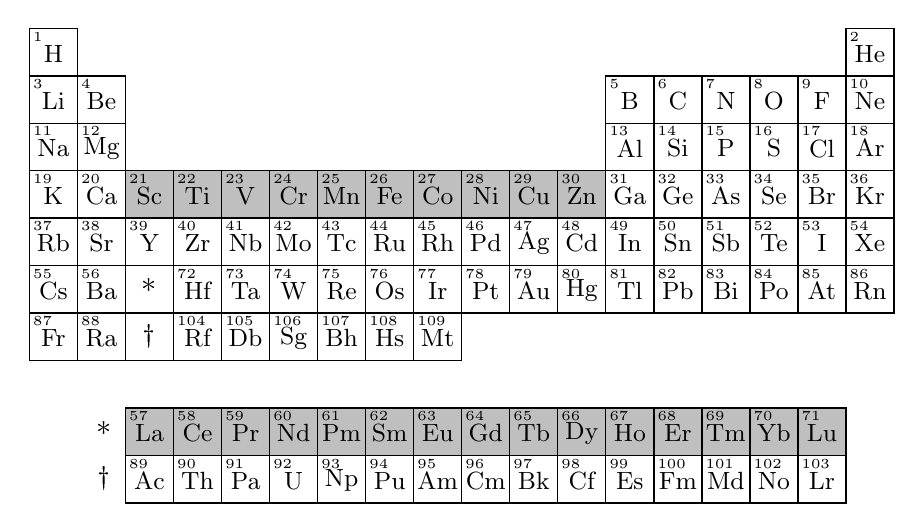
\begin{tikzpicture}[x=0.61cm,y=-0.6026cm,line width=0.5pt]
% ---- shading: 3d row (Sc-Zn) and 4f row (La-Lu) ----
\foreach \c in {3,...,12} \fill[gray!50] (\c-1,3) rectangle (\c,4);
\fill[gray!50] (2,8) rectangle (17,9);
% ---- element cells ----
\foreach \c/\r/\z/\s in {
  1/1/1/H, 18/1/2/He,
  1/2/3/Li, 2/2/4/Be, 13/2/5/B, 14/2/6/C, 15/2/7/N, 16/2/8/O, 17/2/9/F, 18/2/10/Ne,
  1/3/11/Na, 2/3/12/Mg, 13/3/13/Al, 14/3/14/Si, 15/3/15/P, 16/3/16/S, 17/3/17/Cl, 18/3/18/Ar,
  1/4/19/K, 2/4/20/Ca, 3/4/21/Sc, 4/4/22/Ti, 5/4/23/V, 6/4/24/Cr, 7/4/25/Mn, 8/4/26/Fe,
  9/4/27/Co, 10/4/28/Ni, 11/4/29/Cu, 12/4/30/Zn, 13/4/31/Ga, 14/4/32/Ge, 15/4/33/As,
  16/4/34/Se, 17/4/35/Br, 18/4/36/Kr,
  1/5/37/Rb, 2/5/38/Sr, 3/5/39/Y, 4/5/40/Zr, 5/5/41/Nb, 6/5/42/Mo, 7/5/43/Tc, 8/5/44/Ru,
  9/5/45/Rh, 10/5/46/Pd, 11/5/47/Ag, 12/5/48/Cd, 13/5/49/In, 14/5/50/Sn, 15/5/51/Sb,
  16/5/52/Te, 17/5/53/I, 18/5/54/Xe,
  1/6/55/Cs, 2/6/56/Ba, 4/6/72/Hf, 5/6/73/Ta, 6/6/74/W, 7/6/75/Re, 8/6/76/Os, 9/6/77/Ir,
  10/6/78/Pt, 11/6/79/Au, 12/6/80/Hg, 13/6/81/Tl, 14/6/82/Pb, 15/6/83/Bi, 16/6/84/Po,
  17/6/85/At, 18/6/86/Rn,
  1/7/87/Fr, 2/7/88/Ra, 4/7/104/Rf, 5/7/105/Db, 6/7/106/Sg, 7/7/107/Bh, 8/7/108/Hs, 9/7/109/Mt,
  3/9/57/La, 4/9/58/Ce, 5/9/59/Pr, 6/9/60/Nd, 7/9/61/Pm, 8/9/62/Sm, 9/9/63/Eu, 10/9/64/Gd,
  11/9/65/Tb, 12/9/66/Dy, 13/9/67/Ho, 14/9/68/Er, 15/9/69/Tm, 16/9/70/Yb, 17/9/71/Lu,
  3/10/89/Ac, 4/10/90/Th, 5/10/91/Pa, 6/10/92/U, 7/10/93/Np, 8/10/94/Pu, 9/10/95/Am,
  10/10/96/Cm, 11/10/97/Bk, 12/10/98/Cf, 13/10/99/Es, 14/10/100/Fm, 15/10/101/Md,
  16/10/102/No, 17/10/103/Lr%
}{
  \draw (\c-1,\r-1) rectangle (\c,\r);
  \node[anchor=north west,inner sep=1.1pt,
        font=\fontsize{4.8}{5.4}\selectfont] at (\c-1,\r-1) {\z};
  \node[font=\fontsize{8.8}{9.6}\selectfont] at (\c-0.5,\r-0.47) {\s};
}
% ---- asterisk / dagger placeholder cells in rows 6 and 7 ----
\draw (2,5) rectangle (3,6);
\node[font=\fontsize{11}{11}\selectfont] at (2.5,5.42) {$*$};
\draw (2,6) rectangle (3,7);
\node[font=\fontsize{9.5}{9.5}\selectfont] at (2.5,6.48) {\dag};
% ---- asterisk / dagger beside the lanthanide and actinide rows ----
\node[font=\fontsize{11}{11}\selectfont] at (1.55,8.44) {$*$};
\node[font=\fontsize{9.5}{9.5}\selectfont] at (1.55,9.48) {\dag};
\end{tikzpicture}
\end{document}
